\documentclass{article}
\usepackage[T1]{fontenc}
\usepackage{graphicx}
\usepackage{amsmath, amsthm, amssymb}
\usepackage{hyperref}
\usepackage{polski}
\usepackage{array}
\newtheorem{theorem}{Twierdzenie}
\usepackage[a4paper, left=2cm, right=3cm, top=2cm, bottom=2cm]{geometry}
\theoremstyle{definition}
\usepackage{enumerate}
\usepackage{listings}
\usepackage{color}
\newtheorem{definition}{Definicja}

\title{Sprawozdanie Lista1}
\author{Paweł Solecki}
\date{\today}
\begin{document}
	\maketitle

\section{Zadanie 1: Insertion Sort}
	Insertion sort to algorytm sortowania, który działa poprzez iteracyjne wstawianie kolejnych elementów w odpowiednie miejsce w już posortowanej części tablicy.
	\begin{lstlisting}[language=C++, caption={Implementacja Insertion Sort}]
		void insertionSort(int A[], int n) {
			for (int i = 1; i < n; i++) {
				int x = A[i];
				assign_counter++;
				int j = i - 1;
				while (j >= 0 && A[j] > x) {
					assign_counter++;
					compare_counter++;
					A[j + 1] = A[j];
					assign_counter;
					j--;
				}
				A[j + 1] = x;
				assign_counter++;
			}
		}
	\end{lstlisting}
	Modyfikacja Insertion Sort polega na wstawianiu "na raz"dwóch kolejnych elementów tablicy (uprzednio je porównawszy), a jej implementacja wygląda nastepująco:
	\begin{lstlisting}[language=C++, caption={Implementacja Insertion Sort2}]
		void insertionSort2(int A[], int n){
			for (int i=1; i < n - 1; i += 2){
				int a = A[i];
				assign_counter++;
				int b = A[i + 1];
				assign_counter++;
				if (a > b) {
					swap(a, b);
					assign_counter++;
					compare_counter++;
				}
				int j = i - 1;
				while (j >= 0 && A[j] > a) {
					compare_counter++;
					A[j + 1] = A[j];
					j--;
					assign_counter++;
				}
				A[j + 1] = a;
				assign_counter++;
				j = i;
				while (j >= 0 && A[j] > b) {
					compare_counter++;
					A[j + 1] = A[j];
					j--;
					assign_counter++;
				}
				A[j + 1] = b;
				assign_counter++;
			}
			if (n % 2 == 0) {
				int c = A[n - 1];
				assign_counter++;
				int j = n - 2;
				while (j >= 0 && A[j] > c) {
					compare_counter++;
					A[j + 1] = A[j];
					j--;
					assign_counter++;
				}
				A[j + 1] = c;
				assign_counter++;
			}
		}
	\end{lstlisting}
\section{Zadanie 2: Merge Sort}
	Merge sort działa poprzez rekurencyjne dzielenie tablicy na dwie połowy, aż do osiągnięcia pojedynczych elementów, a następnie scala te elementy w uporządkowane pary, tworząc w ten sposób posortowaną tablicę.
	\begin{lstlisting}[language=C++, caption={Implementacja Merge Sort}]
		void merge_sort(int A[], int left, int right) {
			if (left < right) {
				compare_counter++;
				int mid = left + (right - left) / 2;
				
				merge_sort(A, left, mid);
				merge_sort(A, mid + 1, right);
				
				merge(A, left, mid, right);
			}
		}
	\end{lstlisting}
	Możemy zmodyfikować ten algorytm dzieląc tablicę na trzy części zamiast na dwie.
	\begin{lstlisting}[language=C++, caption={Implementacja Merge Sort}]
		void merge_sort_three(int A[], int left, int right) {
			if (left < right) {
				compare_counter++;
				int mid1 = left + (right - left) / 3;         
				int mid2 = left + 2 * (right - left) / 3;     
				
				merge_sort_three(A, left, mid1);
				merge_sort_three(A, mid1 + 1, mid2);
				merge_sort_three(A, mid2 + 1, right);
				
				merge_three(A, left, mid1, mid2, right);
			}
		}
	\end{lstlisting}
\section{Zadanie 3: Heap Sort}
Heap Sort zamienia dane w kopiec, a następnie iteracyjnie wybiera największy (lub najmniejszy) element, aby uzyskać posortowaną listę.
	\begin{lstlisting}[language=C++, caption={Heap Sort}]
		void HEAP_SORT(int A[], int n) {
			BUILD_HEAP(A, n);
			
			for (int i = n - 1; i > 0; i--) {
				assign_counter++;
				swap(A[0], A[i]);
				HEAPIFY(A, 0, i);
			}
		}
	\end{lstlisting}
	Modyfikacja Heap Sort Ternary polega na użyciu zamiast kopców binarnych kopców ternarnych.
	\begin{lstlisting}[language=C++, caption={Heap Sort Ternary}]
	void HEAPIFY_TERNARY(int A[], int i, int n) {
		int largest = i;
		int l = LEFT2(i);
		int m = MIDDLE2(i);
		int r = RIGHT2(i);
		
		compare_counter++;
		if (l < n && A[l] > A[largest]) {
			assign_counter++;
			largest = l;
		}
		
		compare_counter++;
		if (m < n && A[m] > A[largest]) {
			assign_counter++;
			largest = m;
		}
		
		compare_counter++;
		if (r < n && A[r] > A[largest]) {
			assign_counter++;
			largest = r;
		}
		
		compare_counter++;
		if (largest != i) {
			assign_counter++;
			swap(A[i], A[largest]);
			HEAPIFY_TERNARY(A, largest, n);
		}
	}
	
	void BUILD_HEAP_TERNARY(int A[], int n) {
		
		for (int i = n / 3 - 1; i >= 0; i--) {
			HEAPIFY_TERNARY(A, i, n);
		}
	}
	void HEAP_SORT_TERNARY(int A[], int n) {
		BUILD_HEAP_TERNARY(A, n);
		
		for (int i = n - 1; i > 0; i--) {
			assign_counter++;
			swap(A[0], A[i]);
			HEAPIFY_TERNARY(A, 0, i);
		}
	\end{lstlisting}
\section{Zadanie 4: Porównania i Przypisania}
W celu porównania algorytmów i ich modyfikacji przeprowadzono sześć testów na różnych rozmiarach tabeli. Podczas każdego wykonania algorytmu zliczane były porównania i przypisania. Wyniki testów są przedstawione w formie tabel.
	\begin{table}[ht]
		\centering
		\resizebox{\textwidth}{!}{
		\begin{tabular}{|c|c|c|c|c|c|c|}
			\hline
			\textbf{Porównania} & \textbf{insertion\_sort} & \textbf{insertion\_sort2} & \textbf{merge\_sort} & \textbf{merge\_sort\_three} & \textbf{heap\_sort} & \textbf{heap\_sort\_ternary} \\ \hline
			\textbf{Tablica1 (60 elementów)}  & 967  & 985  & 279  & 196  & 993  & 984   \\ \hline
			\textbf{Tablica2 (80 elementów)}  & 1455 & 1470 & 400  & 278  & 1440 & 1412  \\ \hline
			\textbf{Tablica3 (100 elementów)} & 2181 & 2204 & 511  & 356  & 1794 & 1724  \\ \hline
			\textbf{Tablica4 (120 elementów)} & 3340 & 3368 & 635  & 438  & 2184 & 2100  \\ \hline
			\textbf{Tablica5 (140 elementów)} & 4270 & 4299 & 757  & 520  & 2613 & 2460  \\ \hline
			\textbf{Tablica6 (160 elementów)} & 5703 & 5742 & 897  & 609  & 3018 & 2884  \\ \hline
		\end{tabular}
	}
		\caption{Zestawienie ilości porównań w róznych algorytmach sortowania.}
	\end{table}
	\begin{table}[ht]
		\centering
		\resizebox{\textwidth}{!}{
		\begin{tabular}{|c|c|c|c|c|c|c|}
			\hline
			\textbf{Przypisania} & \textbf{insertion\_sort} & \textbf{insertion\_sort2} & \textbf{merge\_sort} & \textbf{merge\_sort\_three} & \textbf{heap\_sort} & \textbf{heap\_sort\_ternary} \\ \hline
			\textbf{Tablica1 (60 elementów)}  & 1085  & 1085  & 712  & 480  & 642  & 494   \\ \hline
			\textbf{Tablica2 (80 elementów)}  & 1613  & 1613  & 1024 & 640  & 946  & 711   \\ \hline
			\textbf{Tablica3 (100 elementów)} & 2371  & 2371  & 1280 & 828  & 1196 & 878   \\ \hline
			\textbf{Tablica4 (120 elementów)} & 3566  & 3566  & 1568 & 1044 & 1443 & 1089  \\ \hline
			\textbf{Tablica5 (140 elementów)} & 4528  & 4528  & 1828 & 1236 & 1742 & 1284  \\ \hline
			\textbf{Tablica6 (160 elementów)} & 5997  & 5997  & 2152 & 1452 & 2025 & 1520  \\ \hline
		\end{tabular}
	}
		\caption{Porównanie ilości przypisań dla różnych algorytmów sortowania.}
	\end{table}
\section{Zadanie 5: Porównanie i Wnioski}
\begin{figure}[h]	
	\includegraphics[width=1.0\textwidth]{wykresporównania2.jpg} 
	\label{fig:wykres porównania}
\end{figure}	

\begin{figure}[h]	
	\centering
	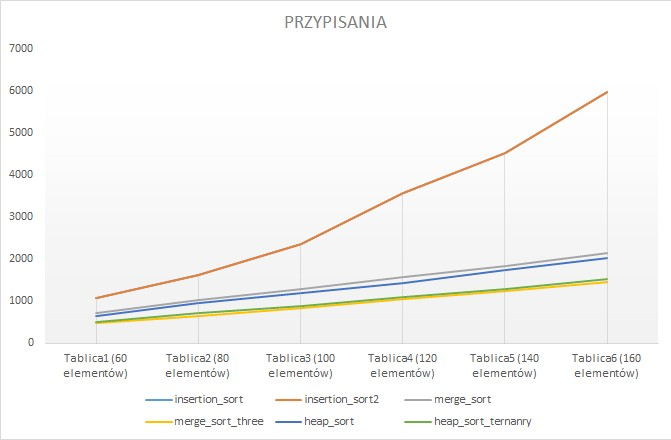
\includegraphics[width=1.0\textwidth]{wykresprzypisania2.jpg} 
	\label{fig:wykres2}
\end{figure}	




Na podstawie wyników testów można zauważyć różnice w efektywności różnych algorytmów sortowania, szczególnie pod kątem liczby porównań i przypisań. Algorytmy sortowania przez wstawianie (insertion sort) w obu wersjach, czyli \texttt{insertion\_sort} i \texttt{insertion\_sort2}, charakteryzują się zbliżoną liczbą porównań i przypisań, co wskazuje na brak istotnych różnic między nimi. W obu przypadkach liczba operacji rośnie proporcjonalnie do rozmiaru tablicy, co jest typowe dla algorytmów o złożoności O($n^2$). Z tego powodu algorytmy te stają się znacznie mniej wydajne przy większych zbiorach danych, o czym świadczy gwałtowny wzrost liczby porównań i przypisań dla tablic o większej liczbie elementów. Przykładowo, dla tablicy zawierającej 160 elementów liczba porównań sięga ponad 5700, a liczba przypisań prawie 6000.

W przypadku algorytmu sortowania przez scalanie (merge sort), zarówno klasyczna wersja, jak i modyfikacja \texttt{merge\_sort\_three}, działają zdecydowanie efektywniej. Złożoność tych algorytmów wynosi O($n \log n$), co przekłada się na znacznie mniejszą liczbę porównań i przypisań w porównaniu do sortowania przez wstawianie. Szczególnie widoczna jest różnica między klasycznym merge sortem a jego wersją trójdzielną. Algorytm \texttt{merge\_sort\_three} wymaga mniej operacji zarówno porównań, jak i przypisań, co czyni go bardziej wydajnym, zwłaszcza w przypadku większych tablic. Na przykład, dla tablicy z 160 elementami liczba porównań w przypadku \texttt{merge\_sort\_three} wynosi zaledwie 609, podczas gdy klasyczny merge sort potrzebuje 897 porównań. Różnica w liczbie przypisań jest również znacząca: 1452 dla wersji trójdzielnej w porównaniu do 2152 w klasycznym merge sorcie.

Algorytm sortowania przez kopcowanie (heap sort) również ma złożoność O($n \log n$), ale w porównaniu do merge sort wypada nieco gorzej pod względem liczby operacji. Wersja trójdzielna heap sort (\texttt{heap\_sort\_ternary}) okazuje się jednak bardziej efektywna niż klasyczny heap sort. Zarówno liczba porównań, jak i przypisań jest mniejsza w tej modyfikacji, co widać szczególnie przy większych rozmiarach tablic. Dla tablicy o 160 elementach, \texttt{heap\_sort\_ternary} wymaga 2884 porównań i 1520 przypisań, podczas gdy klasyczna wersja heap sort wykonuje odpowiednio 3018 porównań i 2025 przypisań.

Podsumowując, algorytmy o złożoności O($n^2$) (\texttt{insertion\_sort}) są znacznie mniej efektywne przy większych tablicach, co potwierdza ich wysoki koszt obliczeniowy. Z kolei algorytmy o złożoności O($n \log n$), takie jak merge sort i heap sort, wypadają znacznie lepiej. Szczególnie korzystne są modyfikacje trójdzielne tych algorytmów (\texttt{merge\_sort\_three} i \texttt{heap\_sort\_ternary}), które wymagają mniejszej liczby operacji, co czyni je bardziej wydajnymi, zwłaszcza w przypadku większych zbiorów danych.

\end{document}